\documentclass[tikz,border=0pt]{standalone}
% rppreamble.tex -- engine switch for the standalone figure builds.
% Tectonic/XeTeX loads xeCJK; pdfLaTeX (arXiv) loads CJKutf8 with gbsn.
% Every Chinese string goes through \zh{...}. main.tex repeats this switch,
% and the standalone package skips this preamble when main.tex inputs a figure.
\usepackage{iftex}
\ifXeTeX
  \usepackage{xeCJK}
  \setCJKmainfont{FandolSong-Regular.otf}
  \setCJKsansfont{FandolHei-Regular.otf}
  \setCJKmonofont{FandolHei-Regular.otf}
  \providecommand{\zh}[1]{#1}
\else
  \usepackage[T1]{fontenc}
  \usepackage[utf8]{inputenc}
  \usepackage{lmodern}
  \usepackage{CJKutf8}
  \DeclareRobustCommand{\zh}[1]{\begin{CJK}{UTF8}{gbsn}#1\end{CJK}}
\fi
\usepackage{amsmath,amssymb}
\usepackage{xcolor}
\usepackage{tikz}
% rpstyle.tex -- the one visual system shared by every ReadProof figure.
% Loaded by each standalone figure (through rppreamble.tex) and by main.tex.
% Palette: ink #03080a for text and plain flow; violet #5b4be8 for ReadProof
% components; red #e2452a for walls and failures; greys for neutral parts.
% Labels are set at 8--8.5 pt so they stay readable at 100% in the paper.
\usetikzlibrary{positioning,arrows.meta,calc,shapes.geometric,shapes.misc,fit,backgrounds}
\definecolor{rpInk}{HTML}{03080A}
\definecolor{rpViolet}{HTML}{5B4BE8}
\definecolor{rpRed}{HTML}{E2452A}
\definecolor{rpGrey}{HTML}{8C929B}
\definecolor{rpGreyDark}{HTML}{50565E}
\definecolor{rpGreyFill}{HTML}{F2F3F5}
\definecolor{rpVioletFill}{HTML}{ECE9FC}
\definecolor{rpVioletPale}{HTML}{F8F7FE}
\definecolor{rpRedFill}{HTML}{FCE9E5}
\providecommand{\rpfont}{\fontsize{8.5}{10}\selectfont\sffamily}
\providecommand{\rpsmall}{\fontsize{8}{9.4}\selectfont\sffamily}
\providecommand{\rpmono}{\fontsize{7.8}{9.2}\selectfont\ttfamily}
\providecommand{\rpdot}{\,\ensuremath{\cdot}\,}
\providecommand{\rpto}{\ensuremath{\rightarrow}}
\providecommand{\rpt}[1]{{\fontsize{8.5}{10.2}\selectfont\bfseries #1}}% node title
\tikzset{
  rp base/.style={rounded corners=3pt, line width=0.6pt, align=center,
    inner xsep=4pt, inner ysep=2.6pt, font=\rpsmall, text=rpInk,
    execute at begin node={\hyphenpenalty=10000\exhyphenpenalty=10000}},
  neutral/.style={rp base, draw=rpGrey, fill=rpGreyFill},
  rp/.style={rp base, draw=rpViolet, fill=rpVioletFill},
  rp strong/.style={rp base, draw=rpViolet, fill=rpViolet, text=white},
  rp gate/.style={rp base, draw=rpViolet, fill=rpVioletFill, line width=1.15pt},
  wall/.style={rp base, draw=rpRed, fill=rpRedFill},
  wall strong/.style={rp base, draw=rpRed, fill=rpRed, text=white},
  data/.style={rp base, draw=rpGrey, fill=white, font=\rpmono, align=left},
  store/.style={cylinder, shape border rotate=90, aspect=0.07, draw=rpViolet,
    fill=rpVioletFill, line width=0.6pt, align=center, font=\rpsmall,
    text=rpInk, inner xsep=4pt, inner ysep=1pt,
    execute at begin node={\hyphenpenalty=10000\exhyphenpenalty=10000}},
  flow/.style={-{Stealth[length=5pt,width=4pt]}, line width=0.7pt, draw=rpInk},
  rpflow/.style={flow, draw=rpViolet},
  wallflow/.style={flow, draw=rpRed},
  logflow/.style={-{Stealth[length=4pt,width=3.5pt]}, line width=0.55pt,
    draw=rpGrey, dash pattern=on 2.6pt off 1.8pt},
  assoc/.style={line width=0.7pt, draw=rpViolet},
  edge label/.style={font=\rpsmall, text=rpGreyDark, inner sep=1.2pt},% no fill: place clear of lines
  wall label/.style={edge label, text=rpRed, fill=white},% white patch: may sit across a panel border
  group/.style={rounded corners=6pt, draw=rpViolet!35, fill=rpVioletPale,
    line width=0.5pt},
  group label/.style={font=\rpsmall\bfseries, text=rpViolet},
  panel title/.style={font=\fontsize{9}{11}\selectfont\sffamily\bfseries, text=rpInk},
}

% Opaque white page under everything, for the standalone PDFs and PNG checks
% only (main.tex never reads this preamble). A layer below "background" keeps
% the pale group panels visible.
\pgfdeclarelayer{rppage}
\pgfsetlayers{rppage,background,main}
\tikzset{every picture/.append style={execute at end picture={%
  \begin{pgfonlayer}{rppage}\fill[white]
    ([shift={(-2pt,-2pt)}]current bounding box.south west) rectangle
    ([shift={(2pt,2pt)}]current bounding box.north east);\end{pgfonlayer}}}}

\begin{document}
% How ReadProof-Bench is built: five steps (columns) x track rows.
% Rows: Track A (y=6.48), Track B (4.29), Track C (2.23), Track K (0).
% Panels: P1 [0,2.56] P2 [2.86,6.04] P3 [6.24,9.32] P4 [9.62,12.44] P5 [12.74,15.25].
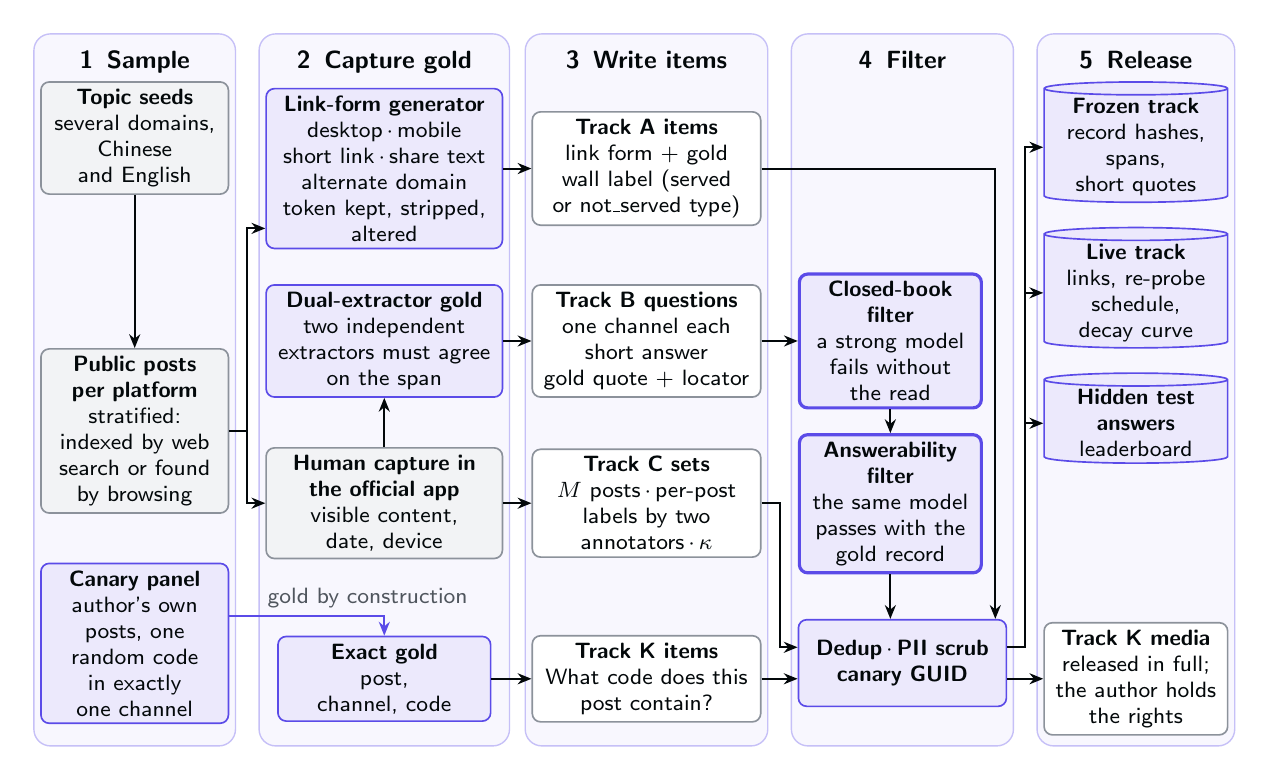
\begin{tikzpicture}[
  item/.style={data, font=\rpsmall, align=center},
]
\def\yA{6.48}\def\yB{4.29}\def\yC{2.23}\def\yK{0}
\def\yRun{0.8}% violet canary arrow
\def\yD{0.2}% dedup centre
% ---------------- 1 Sample ----------------
\node[neutral, text width=2.1cm, anchor=north] (TS) at (1.28,7.59)
  {\rpt{Topic seeds}\\several domains,\\Chinese and English};
\node[neutral, text width=2.1cm, anchor=north] (PP) at (1.28,4.2)
  {\rpt{Public posts}\\\rpt{per platform}\\stratified:\\indexed by web\\search or found\\by browsing};
\node[rp, text width=2.1cm] (CP) at (1.28,0.45)
  {\rpt{Canary panel}\\author's own\\posts, one\\random code\\in exactly\\one channel};
% ---------------- 2 Capture gold ----------------
\node[rp, text width=2.72cm] (LF) at (4.45,\yA)
  {\rpt{Link-form generator}\\desktop\rpdot mobile\\short link\rpdot share text\\alternate domain\\token kept, stripped,\\altered};
\node[rp, text width=2.72cm] (DX) at (4.45,\yB)
  {\rpt{Dual-extractor gold}\\two independent\\extractors must agree\\on the span};
\node[neutral, text width=2.72cm] (HC) at (4.45,\yC)
  {\rpt{Human capture in}\\\rpt{the official app}\\visible content,\\date, device};
\node[rp, text width=2.42cm] (EG) at (4.45,\yK)
  {\rpt{Exact gold}\\post, channel, code};
% ---------------- 3 Write items ----------------
\node[item, text width=2.62cm] (IA) at (7.78,\yA)
  {\rpt{Track A items}\\link form + gold\\wall label (served\\or not\_served type)};
\node[item, text width=2.62cm] (IB) at (7.78,\yB)
  {\rpt{Track B questions}\\one channel each\\short answer\\gold quote + locator};
\node[item, text width=2.62cm] (IC) at (7.78,\yC)
  {\rpt{Track C sets}\\$M$ posts\rpdot per-post\\labels by two\\annotators\rpdot $\kappa$};
\node[item, text width=2.62cm] (IK) at (7.78,\yK)
  {\rpt{Track K items}\\What code does this\\post contain?};
% ---------------- 4 Filter ----------------
\node[rp gate, text width=2.03cm] (CB) at (10.877,\yB)
  {\rpt{Closed-book}\\\rpt{filter}\\a strong model\\fails without\\the read};
\node[rp gate, text width=2.03cm, anchor=north] (AN) at ($(CB.south)+(0,-0.3)$)
  {\rpt{Answerability}\\\rpt{filter}\\the same model\\passes with the\\gold record};
\node[rp, text width=2.36cm, minimum height=1.1cm] (DD) at (11.03,\yD)
  {\rpt{Dedup\rpdot PII scrub}\\\rpt{canary GUID}};
% ---------------- 5 Release ----------------
\node[store, text width=2.05cm, anchor=north] (FT) at (13.995,7.59)
  {\rpt{Frozen track}\\record hashes,\\spans,\\short quotes};
\node[store, text width=2.05cm, anchor=north] (LT) at ($(FT.south)+(0,-0.3)$)
  {\rpt{Live track}\\links, re-probe\\schedule,\\decay curve};
\node[store, text width=2.05cm, anchor=north] (HT) at ($(LT.south)+(0,-0.3)$)
  {\rpt{Hidden test}\\\rpt{answers}\\leaderboard};
\node[item, text width=2.05cm] (KM) at (13.995,\yK)
  {\rpt{Track K media}\\released in full;\\the author holds\\the rights};
% ---------------- flows ----------------
\draw[flow] (TS) -- (PP);
\draw[flow] (PP.east) -- (2.71,0|-PP.east) |- (HC.west);
\draw[flow] (PP.east) -- (2.71,0|-PP.east) |- (LF.west|-0,5.72);
\draw[flow] (LF.east|-0,\yA) -- (IA.west|-0,\yA);
\draw[flow] (HC) -- (DX);
\draw[flow] (DX) -- (IB);
\draw[flow] (HC) -- (IC);
\draw[rpflow] (CP.east|-0,\yRun) -| (EG.north);
\node[edge label, anchor=south west] at (2.92,\yRun+0.05) {gold by construction};
\draw[flow] (EG) -- (IK);
\draw[flow] (IB) -- (CB);
\draw[flow] (CB) -- (AN);
\draw[flow] (AN.south) -- (AN.south|-DD.north);
\draw[flow] (IC.east) -- (9.47,\yC) |- (DD.west|-0,0.4);
\draw[flow] (IK.east) -- (DD.west|-0,\yK);
\draw[flow] (IA.east) -- (12.21,\yA) -- (12.21,0|-DD.north);
\foreach \s in {FT,LT,HT}{\draw[flow] (DD.east|-0,0.4) -- (12.59,0.4) |- (\s.west);}
\draw[flow] (DD.east|-0,\yK) -- (KM.west|-0,\yK);
% ---------------- panels and headers ----------------
\path let \p1=(current bounding box.north), \p2=(current bounding box.south) in
  coordinate (top) at (0,\y1+0.6cm) coordinate (bot) at (0,\y2-0.13cm);
\begin{scope}[on background layer]
  \foreach \l/\r in {0/2.56, 2.86/6.04, 6.24/9.32, 9.62/12.44, 12.74/15.25}
    {\path[group] (\l,0|-bot) rectangle (\r,0|-top);}
\end{scope}
\foreach \x/\t in {1.28/1\enspace Sample, 4.45/2\enspace Capture gold, 7.78/3\enspace Write items,
                   11.03/4\enspace Filter, 13.995/5\enspace Release}
  {\node[panel title, anchor=north] at ($(\x,0|-top)+(0,-0.1)$) {\t};}
\end{tikzpicture}
\end{document}
